\documentclass[english]{exam}

\setlength {\marginparwidth }{2cm} 
\usepackage{todonotes}

\usepackage[perpage,para,symbol]{footmisc}

\hyphenpenalty=15000 
\tolerance=1000

\usepackage{tikz}
\usetikzlibrary{arrows,decorations.pathmorphing,backgrounds,fit,positioning,calc,shapes}
\usepackage{pgfmath}
\usepackage{rotating}
\usepackage{array}	
\usepackage{graphicx}
\usepackage{float}	
\usepackage{mdwlist}
\usepackage{setspace}
\usepackage{listings}
\usepackage{bytefield}
\usepackage{tabularx}
\usepackage{multirow}	       
\usepackage{caption}
\usepackage{amssymb}
\captionsetup[table]{skip=10pt}

\usepackage{url}               
\usepackage{hyperref}
\usepackage[all]{hypcap}	
\usepackage{titlesec}
\setcounter{secnumdepth}{4}
\titleformat{\paragraph}
{\normalfont\normalsize\bfseries}{\theparagraph}{1em}{}
\titlespacing*{\paragraph}
{0pt}{3.25ex plus 1ex minus .2ex}{1.5ex plus .2ex}
\hypersetup{colorlinks,breaklinks,
            linkcolor=darkblue,urlcolor=darkblue,
            anchorcolor=darkblue,citecolor=darkblue}


\definecolor{darkblue}{rgb}{0.0,0.0,0.3} 
\definecolor{darkred}{rgb}{0.4,0.0,0.0}
\definecolor{red}{rgb}{0.7,0.0,0.0}
\definecolor{lightgrey}{rgb}{0.8,0.8,0.8} 
\definecolor{grey}{rgb}{0.6,0.6,0.6}
\definecolor{darkgrey}{rgb}{0.4,0.4,0.4}
\definecolor{aqua}{rgb}{0.0, 1.0, 1.0}
\definecolor{dkgreen}{rgb}{0,0.6,0}
\definecolor{gray}{rgb}{0.5,0.5,0.5}
\definecolor{mauve}{rgb}{0.58,0,0.82}

\lstset{
  language=C,
  showstringspaces=false,
  columns=flexible,
  basicstyle={\small\ttfamily},
  numbers=none,
  numberstyle=\tiny\color{gray},
  keywordstyle=\color{blue},
  commentstyle=\color{dkgreen},
  stringstyle=\color{mauve},
  breaklines=true,
  breakatwhitespace=true,
  tabsize=3
}
\usepackage{listings}
\PassOptionsToPackage{USenglish,english}{babel} 
\usepackage{csquotes}
\usepackage[USenglish,english]{babel}
\usepackage[acronym, section=section, nonumberlist, nomain, nopostdot]{glossaries}
\makeglossaries
 
\makeglossaries
\newcommand{\colorbitbox}[3]{%
	\rlap{\bitbox{#2}{\color{#1}\rule{\width}{\height}}}%
	\bitbox{#2}{#3}}

\begin{document}

\title{Assignment I:\\ GPU Architectures and Accelerators}
\author{Amirhossein Namazi, Calin Capitanu}

\maketitle


\chapter{Exercise 1}
\section*{Questions about GPU Architectures and Accelerators}

\begin{enumerate}
\item Why GPUs has emerged as suitable hardware for computer graphics (e.g. games)?\\\\
  GPUs were created in order to perform good in parallel problems that also do not require synchronization. The performance they achieve in such problems, together with their FLOPS/Watt ratio is are the key factors that allowed GPUs to emerge so rapidly in the market for such problems, such as games, which require a lot of graphical computation and image processing.
\item Why do we talk about throughput-oriented architecture when we talk about GPUs?\\\\
Since throughput-oriented architectures highly increase the parallelization possibilities and also since we are not looking for dependable processing, GPUs are naturally focusing on throughput-oriented architectures. A high number of physical cores and hardware threading allows for all of this parallelization and also endorse the architecture mentioned.  
\item List the main differences between GPUs and CPUs in terms of architecture.
  \begin{enumerate}
  \item The GPU architecture has more multiprocessors, whereas the CPU usually only has one (however, there are changes in the new architectures of AMD processors towards multiple multi-processors, but that is still fundamentally different!).
  \item The GPU multi-cores usually contain a lot more cores, and those cores are really basic, while the CPU cores are more complex.
  \item in GPU architecture, each SM handles its own thread management in hardware with the use of SIMT units.
  \end{enumerate}
\item Use the Internet to find out and list the number of SMs, the number of cores per SM, the clock frequency, and the size of the memory of the NVIDIA GPU that you plan to use during the course. It might be the GPU of your laptop/workstation or the GPUs on Tegner (Links to an external site.) (NVIDIA Quadro K420 or NVIDIA Tesla K80). Please, make sure that you mention the specific model as well.\\\\
  During this course I will be using the NVIDIA RTX 3080 GPU of my own computer. The specifications are:
  \begin{itemize}
  \item Number of SMs: 68
  \item Cores per SM: 128 cores
  \item Clock Frequency: 1440 MHz (base), 1935 MHz (overclocked)
  \item Memory Size: 10GB GDDR6X
  \end{itemize}
  
\item Volta introduced Tensor cores.
  \begin{enumerate}
  \item Which operation does the Tensor core support in one clock cycle?\\
    Tensor cores can calculate matrix multiplication and addition of small 4x4 matrices. That is, tensor cores can compute $C = C + A * B$, where A,B and C are 4x4 matrices.
  \item What is the precision supported by Tensor cores?\\
    Tensor cores have a precision of maximum 125 TFLOPS/s with low precision.
  \item Why do you think that Tensor Cores were introduced in the new GPUs? For graphics or other applications?\\
    The initial thought is that Machine Learning uses matrix multiplication at a high extent, thus the introduction of this feature in the core unit of a GPU would highly benefit this field.
  \end{enumerate}
\item Check the Top500 list (Links to an external site.) that is reporting the 500 most powerful supercomputers in the world. How many of the first 10 most powerful supercomputers use GPUs? Report the name of the supercomputers and the GPU vendor (Nvidia, AMD, ...) and model.
  \begin{itemize}
  \item Summit - NVIDIA
  \item Sierra - NVIDIA
  \item HPC5 - NVIDIA
  \item Selene - NVIDIA
  \item Frontera - NVIDIA
  \item Marconi-100 - NVIDIA
  \item Piz Daint - NVIDIA
  \end{itemize}
\item Which upcoming supercomputer will feature AMD GPUs? List at least the names of four supercomputers with AMD GPUs.
  \begin{itemize}
  \item Frontier
  \item El Capitan
  \item LUMI (Large Unified Modern Infrastructure)
  \item Setnoix
  \item Dardel
  \end{itemize}
\item What is an FPGA? What are his advantages and disadvantages?\\\\
  FPGAs (Field Programmable Gate Arrays) are middle ground between highly specialized ASICs and general purpose CPUs. The idea behind them is that hardware can be reprogrammable using CLBs (Configurable Logig Blocks). The architecture is generally consisting of a matrix of CLBs. \\
  As an advantage, FPGAs are designed to receive and transmit signals fast, while at the same time it consumes less power. One disadantage could be the programming environment and the programmability of such chips. It takes special tools to program FPGAs.
  
\item What is an ASIC and what is the Google ASIC for deep-learning calculations? Which architecture the Google's ASIC uses for calculating the matrix multiply? \\
  Google created the TPU (Tensor Processing Unit) for neural networks and deep learning. This TPU uses systolic arrays to compute 8-bit 256x256 multiply-add operations.
  
\item Use Google Scholar to find a scientific paper reporting about a work using GPUs in your main domain area (HPC, image processing, machine learning, ...). Report the title, authors, conference name/journal, the GPU type that has been used, and which programming approach has been employed.\\\\
  ``Performance Prediction of GPU-based Deep Learning Applications'' by Eugenio Gianniti, Li Zhang and Danilo Ardagna. Published in 2018 30th International Symposium on Computer Architecture and High Performance Computing (SBAC-PAD). They use an Nvidia Quattro M6000 and the programming approach is using neural networks to predict performance of predictions of other neural networks, basically analysis.

  
\end{enumerate}

\clearpage

\chapter{Exercise 2}
\section*{Bandwidth Test GPU-CPU}

\begin{lstlisting}
  [CUDA Bandwidth Test] - Starting...
Running on...

 Device 0: NVIDIA GeForce RTX 3080
 Quick Mode

 Host to Device Bandwidth, 1 Device(s)
 PINNED Memory Transfers
   Transfer Size (Bytes)	Bandwidth(GB/s)
   32000000			25.1

 Device to Host Bandwidth, 1 Device(s)
 PINNED Memory Transfers
   Transfer Size (Bytes)	Bandwidth(GB/s)
   32000000			24.6

 Device to Device Bandwidth, 1 Device(s)
 PINNED Memory Transfers
   Transfer Size (Bytes)	Bandwidth(GB/s)
   32000000			578.9

Result = PASS

NOTE: The CUDA Samples are not meant for performance measurements. Results may vary when GPU Boost is enabled.

\end{lstlisting}

\begin{figure}[h]
\centerline{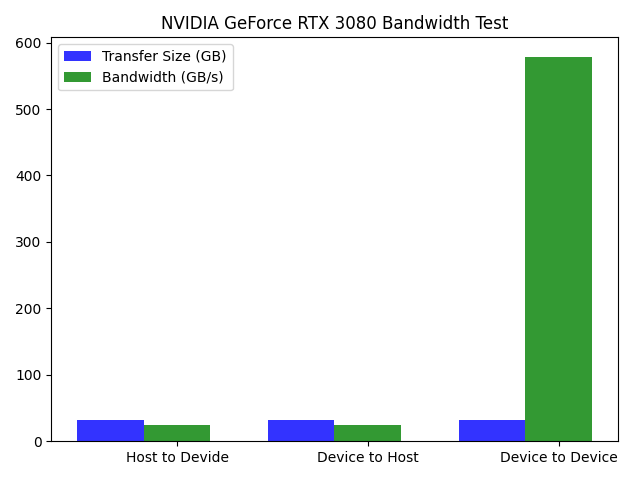
\includegraphics[scale=0.5]{plt1.png}}
\caption{Bandwidth Test}
\label{fig}
\end{figure}

\noindent
The main idea behind this test is to prove that data communication is best done inside the device, but not between the device and the host device. The main reason behind this is that the communication between the device and the host is done through PCIe busses which, however good they might be, they are still limited compared to the one inside the device. The plot above clearly shows that the bandwidth of the device with its own memory is around 20 times better than host to device, while both host to device and device to host are really close to eachother (since they run the same bus lines).


\begin{figure}[h]
\centerline{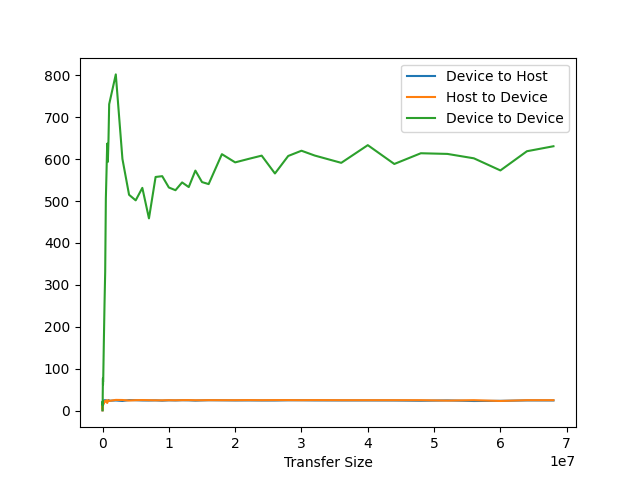
\includegraphics[scale=0.5]{plt2.png}}
\caption{Bandwidth Test}
\label{fig}
\end{figure}

\noindent
The main difference here with the second plot and data is that data is inspected as the transfer size grows. We can see that communication between the host and the device tops of at the same amount as the previous tests show, however when the GPU is communicating with its own memory, the bandwidth is impressingly higher than that and somewhat less constant, but still tops off at around 500-600 GB/s.
\\\\
All the data was extracted from the CUDA tests available below and plotted in graphs for better interpretation and visualization.

\begin{lstlisting}
  [CUDA Bandwidth Test] - Starting...
Running on...

 Device 0: NVIDIA GeForce RTX 3080
 Shmoo Mode

.................................................................................
 Host to Device Bandwidth, 1 Device(s)
 PINNED Memory Transfers
   Transfer Size (Bytes)	Bandwidth(GB/s)
   1000				0.6
   2000				1.2
   3000				2.0
   4000				2.5
   5000				2.8
   6000				3.6
   7000				4.2
   8000				4.0
   9000				5.1
   10000			5.5
   11000			5.2
   12000			6.3
   13000			6.7
   14000			6.1
   15000			7.5
   16000			7.3
   17000			7.0
   18000			8.5
   19000			6.4
   20000			7.5
   22000			10.0
   24000			10.1
   26000			10.7
   28000			9.4
   30000			11.4
   32000			11.9
   34000			10.3
   36000			12.7
   38000			12.9
   40000			10.8
   42000			14.3
   44000			13.7
   46000			14.1
   48000			11.8
   50000			13.7
   60000			15.7
   70000			12.3
   80000			18.4
   90000			18.2
   100000			17.9
   200000			16.5
   300000			22.7
   400000			22.4
   500000			21.4
   600000			24.9
   700000			18.2
   800000			24.4
   900000			24.6
   1000000			23.2
   2000000			25.6
   3000000			25.4
   4000000			24.2
   5000000			25.0
   6000000			25.3
   7000000			25.0
   8000000			24.7
   9000000			24.7
   10000000			25.0
   11000000			24.8
   12000000			25.1
   13000000			25.2
   14000000			24.9
   15000000			24.9
   16000000			25.1
   18000000			25.0
   20000000			25.0
   22000000			25.2
   24000000			25.0
   26000000			25.2
   28000000			25.2
   30000000			25.0
   32000000			25.2
   36000000			25.0
   40000000			25.0
   44000000			25.0
   48000000			25.0
   52000000			24.0
   56000000			25.0
   60000000			23.1
   64000000			25.0
   68000000			25.0

.................................................................................
 Device to Host Bandwidth, 1 Device(s)
 PINNED Memory Transfers
   Transfer Size (Bytes)	Bandwidth(GB/s)
   1000				0.7
   2000				1.4
   3000				2.0
   4000				2.8
   5000				3.4
   6000				4.2
   7000				4.8
   8000				5.5
   9000				6.2
   10000			6.8
   11000			7.5
   12000			9.7
   13000			9.0
   14000			9.7
   15000			10.4
   16000			11.1
   17000			8.5
   18000			9.0
   19000			11.5
   20000			10.1
   22000			12.7
   24000			12.9
   26000			11.0
   28000			11.4
   30000			15.1
   32000			16.0
   34000			15.3
   36000			16.0
   38000			14.2
   40000			13.1
   42000			11.9
   44000			16.8
   46000			17.4
   48000			18.1
   50000			13.8
   60000			14.7
   70000			16.1
   80000			20.6
   90000			21.7
   100000			22.3
   200000			24.4
   300000			23.8
   400000			25.0
   500000			24.5
   600000			24.2
   700000			21.2
   800000			22.5
   900000			25.3
   1000000			23.6
   2000000			24.3
   3000000			23.1
   4000000			25.2
   5000000			24.9
   6000000			24.3
   7000000			24.2
   8000000			24.5
   9000000			23.8
   10000000			24.6
   11000000			24.3
   12000000			24.8
   13000000			24.6
   14000000			23.9
   15000000			24.4
   16000000			24.8
   18000000			24.6
   20000000			24.3
   22000000			24.4
   24000000			24.2
   26000000			24.2
   28000000			24.7
   30000000			24.7
   32000000			24.4
   36000000			24.3
   40000000			24.3
   44000000			24.2
   48000000			23.6
   52000000			24.4
   56000000			23.0
   60000000			23.4
   64000000			24.4
   68000000			24.3

.................................................................................
 Device to Device Bandwidth, 1 Device(s)
 PINNED Memory Transfers
   Transfer Size (Bytes)	Bandwidth(GB/s)
   1000				1.3
   2000				2.7
   3000				3.9
   4000				5.2
   5000				6.5
   6000				7.8
   7000				9.1
   8000				10.3
   9000				11.6
   10000			13.0
   11000			14.2
   12000			15.7
   13000			16.8
   14000			13.2
   15000			14.3
   16000			15.2
   17000			16.1
   18000			17.1
   19000			17.9
   20000			19.1
   22000			21.3
   24000			22.3
   26000			16.4
   28000			36.2
   30000			38.8
   32000			41.7
   34000			44.0
   36000			46.6
   38000			49.2
   40000			51.7
   42000			54.3
   44000			56.9
   46000			59.5
   48000			61.7
   50000			64.2
   60000			77.1
   70000			62.0
   80000			70.3
   90000			69.7
   100000			70.5
   200000			166.6
   300000			255.4
   400000			331.5
   500000			505.8
   600000			569.3
   700000			637.0
   800000			593.5
   900000			648.0
   1000000			731.1
   2000000			802.2
   3000000			600.5
   4000000			515.0
   5000000			501.7
   6000000			531.5
   7000000			458.7
   8000000			557.5
   9000000			559.4
   10000000			532.4
   11000000			525.9
   12000000			544.5
   13000000			533.4
   14000000			572.7
   15000000			545.3
   16000000			540.5
   18000000			611.9
   20000000			592.3
   22000000			600.5
   24000000			608.4
   26000000			565.8
   28000000			607.6
   30000000			620.1
   32000000			608.6
   36000000			591.2
   40000000			633.4
   44000000			588.5
   48000000			614.1
   52000000			612.5
   56000000			602.0
   60000000			573.1
   64000000			618.9
   68000000			630.8

Result = PASS

NOTE: The CUDA Samples are not meant for performance measurements. Results may vary when GPU Boost is enabled.


\end{lstlisting}


\bibliographystyle{myIEEEtran}
\renewcommand{\bibname}{References}
\addcontentsline{toc}{chapter}{References}
\bibliography{references}

\end{document}
